
\section{Modeling as Markov}

\begin{frame}
    \frametitle{Table of contents}
    \tableofcontents
\end{frame} 


\subsection{Markov Chains}
\begin{frame}
    \frametitle{Markov Processes}

    \begin{itemize}
        \item Markov decision process formally describe an environment
        for reinforcement learning;

        \item Where the environment is {\color{red}fully observable};
        \begin{itemize}
            \item The current state completely characterises the process;
        \end{itemize}
        \item Almost all RL problems can be formalised as MDPs:
        \begin{itemize}
            \item Partially observable problems can be converted into MDPs.
        \end{itemize}
    \end{itemize} 

\end{frame}






\begin{frame}
    \frametitle{Markov Property}
    \centering
    {\color{red}The future is independent of the past given the present.}


    \begin{definition}
        A state $S_t$ is Markov if only if
        $$P[S_{t+1}|S_t] = P[S_{t+1}|S_t,S_{t-1},...,S_2,S_1]$$
    \end{definition}

    \begin{itemize}
        \item A Markov process (or Markov Chain) is a memoryless random process;
        \item The state is a sufficient statistic of the future.
    \end{itemize}

\end{frame}


\begin{frame}
    \frametitle{State Transition Matrix}

    For a Markov state $s$ and successor state $s'$, the state Transition
    probability us defined by:

    $$\mathcal{P}_{ss'} = P[S_{t+1}=s'|S_t=s]$$

    We can define the state transition matrix \mathcal{P} defines transition 
    probabilities from all states $s$ to all successor states $s'$

\end{frame}



\begin{frame}
    \frametitle{Example: Weather Markov Chain}
    \begin{figure}
        \centering
        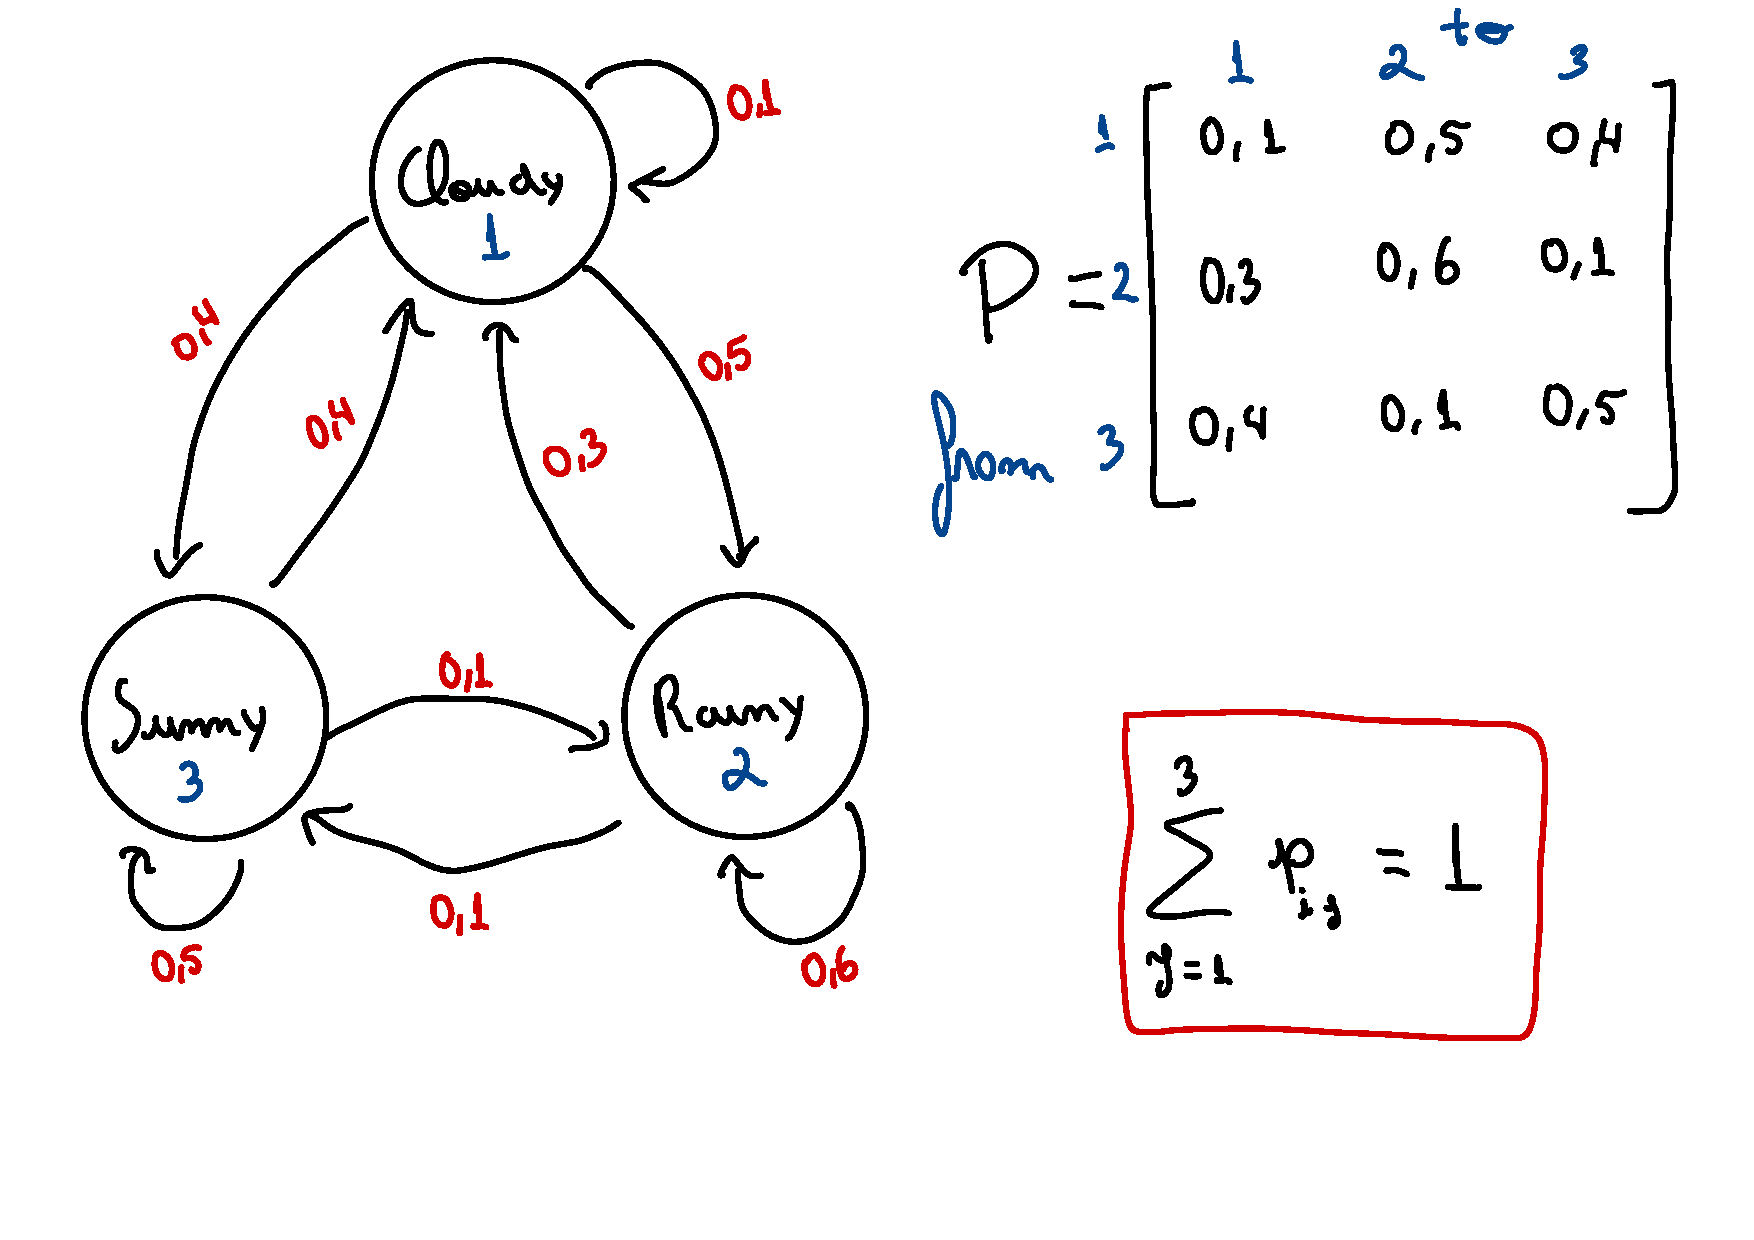
\includegraphics[width=1\textwidth]{sections/markov/figures/weather_markov_chain_01.pdf}
    \end{figure}
\end{frame}



\begin{frame}
    \frametitle{Example: Weather Markov Chain}

    \begin{columns}
        % Column 1
        \begin{column}{0.5\textwidth}
            \begin{figure}
                \centering
                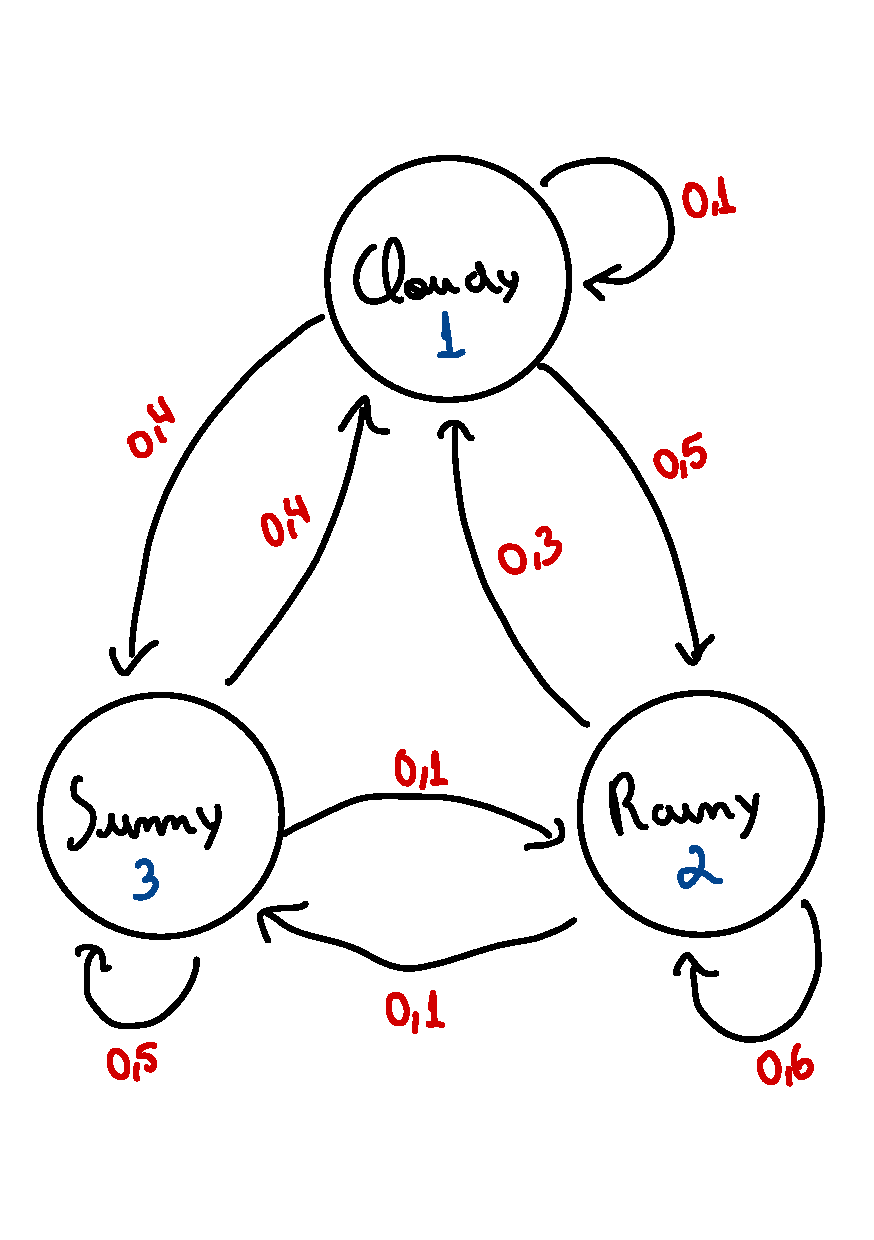
\includegraphics[width=1\textwidth]{sections/markov/figures/weather_markov_chain_02.pdf}
            \end{figure}
        \end{column}

        % Column 2    
        \begin{column}{0.5\textwidth}

            Sample episodes for weather Markov Chain starting from $S_1 = R$ (Rainy).

            $$S_1,S_2,...,S_t$$

            {\color{red}Episodes} is a sequence of states;

            \begin{itemize}
                \item R C S S C;
                \item R R C C S;
                \item R S C C R;
            \end{itemize}  
        \end{column}

    \end{columns}

\end{frame}

\subsection{Markov Reward Process}
\begin{frame}
    \frametitle{Markov Reward Process}
    It is a Markov Chain with values.
    \begin{definition}
        A Markov Reward Process is a tuple $\langle\mathcal{S},\mathcal{P},
        {\color{red}\mathcal{R},\gamma}\rangle$
        \begin{itemize}
            \item $\mathcal{S}$ is a finite set of {\color{red}states};

            \item $\mathcal{P}$ is a {\color{red}transition probability matrix};

            \item $\mathcal{R}$ is a {\color{red}reward function} ($\mathcal{R}_s = \E[R_{t+1}|S_t=s]$);

            \item $\gamma$ is a {\color{red} discount factor}, where $\gamma \in [0,1]$.
        \end{itemize}
    \end{definition}
\end{frame}

\subsubsection{Return}

\begin{frame}
    \frametitle{Return}
 
    \centering
    {\color{red}Return refers to the total discounted reward, starting from the current timestep.}

    \begin{definition}
        The return $G_t$ is the total discounted reward from time-step $t$.
        $$G_t = R_{t+1} + \gammaR_{t+2} + \gamma^{2}R_{t+3} + ... = \sum_{k=0}^{\infty}\gamma^{k}R_{t+k+1}$$
        \begin{itemize}
            \item The discount $\gamma\in[0,1]$ is the present value of future rewards.
        \end{itemize}
    \end{definition}

\end{frame}

\subsubsection{Value Function}

\begin{frame}
    \frametitle{Value Function}
    \centering
    {\color{red}The value function $v(s)$ gives the long-term value of state $s$.}

    \begin{definition}
        The state value function $v(s)$ of a MRP is the expected return starting from state $s$
        $$v(s)=\E[G_t|S_t=s]$$
    \end{definition}
\end{frame}



\begin{frame}
    \frametitle{Value Function (Bellman Equation)}
    The value function can be decomposed into two parts:
    \begin{itemize}
        \item Imediate reward $R_{t+1}$;
        \item Discounted value of successor state $\gammav(S_{t+1})$
    \end{itemize}

    \begin{figure}
        \centering
        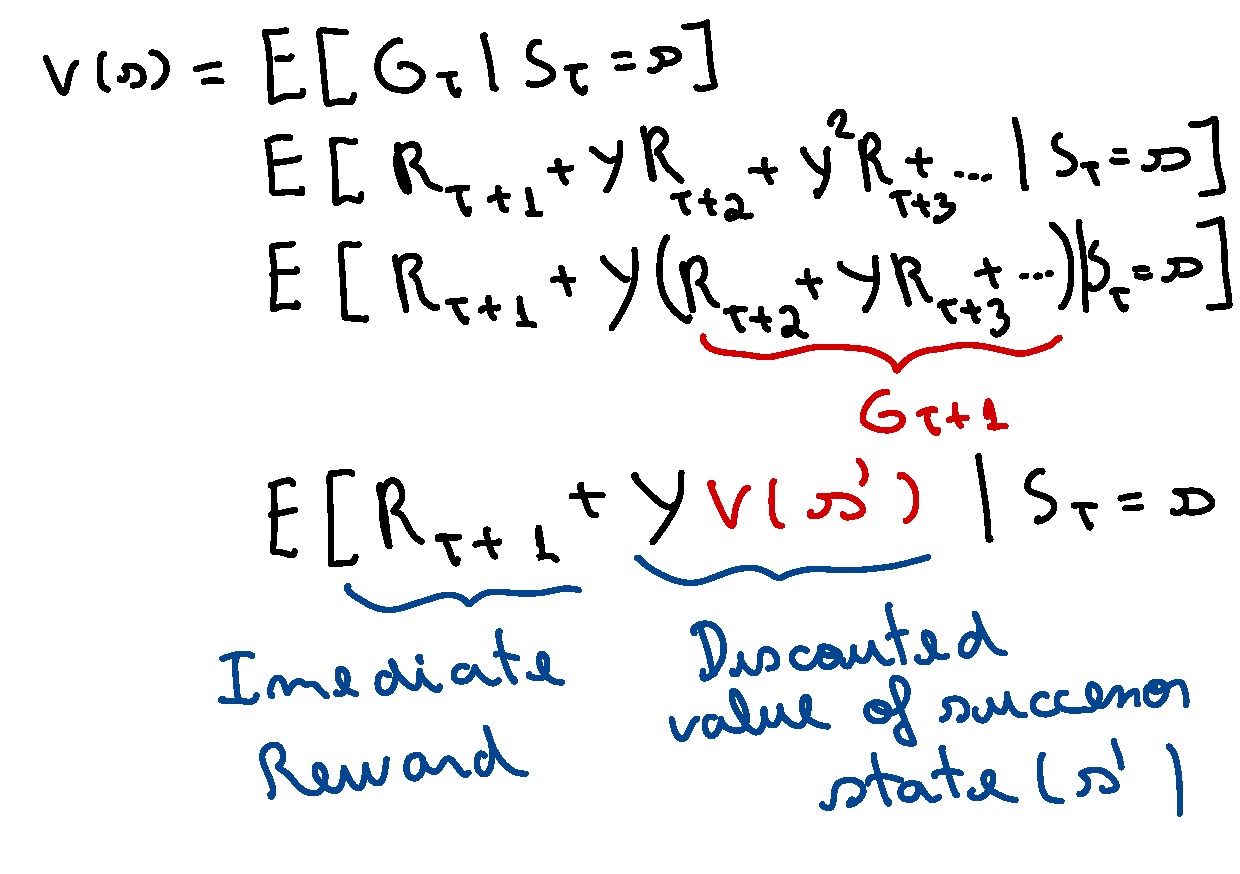
\includegraphics[width=0.7\textwidth]{sections/markov/figures/v_s.pdf}
    \end{figure}

\end{frame}

\begin{frame}
    \frametitle{Value Function (Bellman Equation)}
    The Bellman equation is a linea equation.
    \begin{figure}
        \centering
        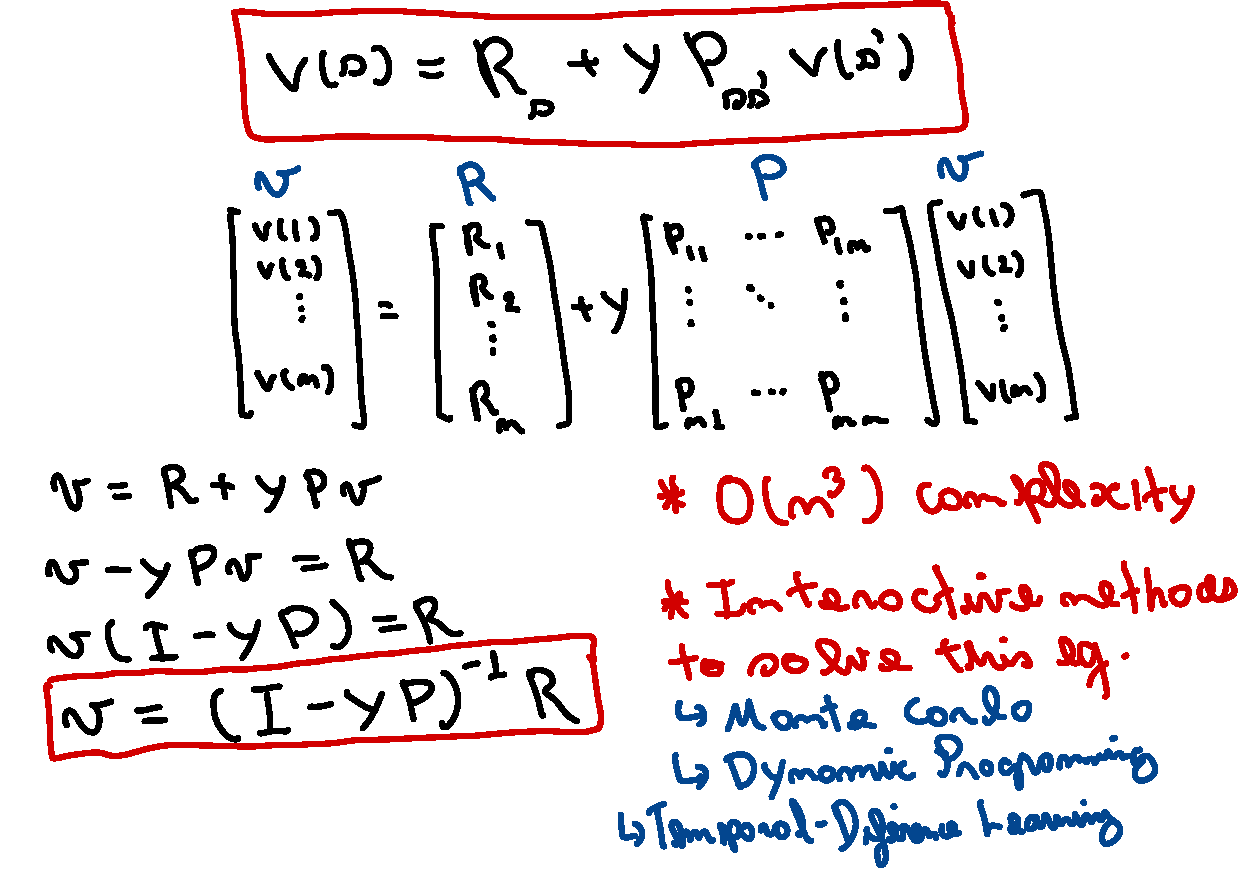
\includegraphics[width=0.9\textwidth]{sections/markov/figures/bellman_eq_matrix_form.pdf}
    \end{figure}

\end{frame}


\begin{frame}
    \frametitle{Value Function (Example)}
    \begin{figure}
        \centering
        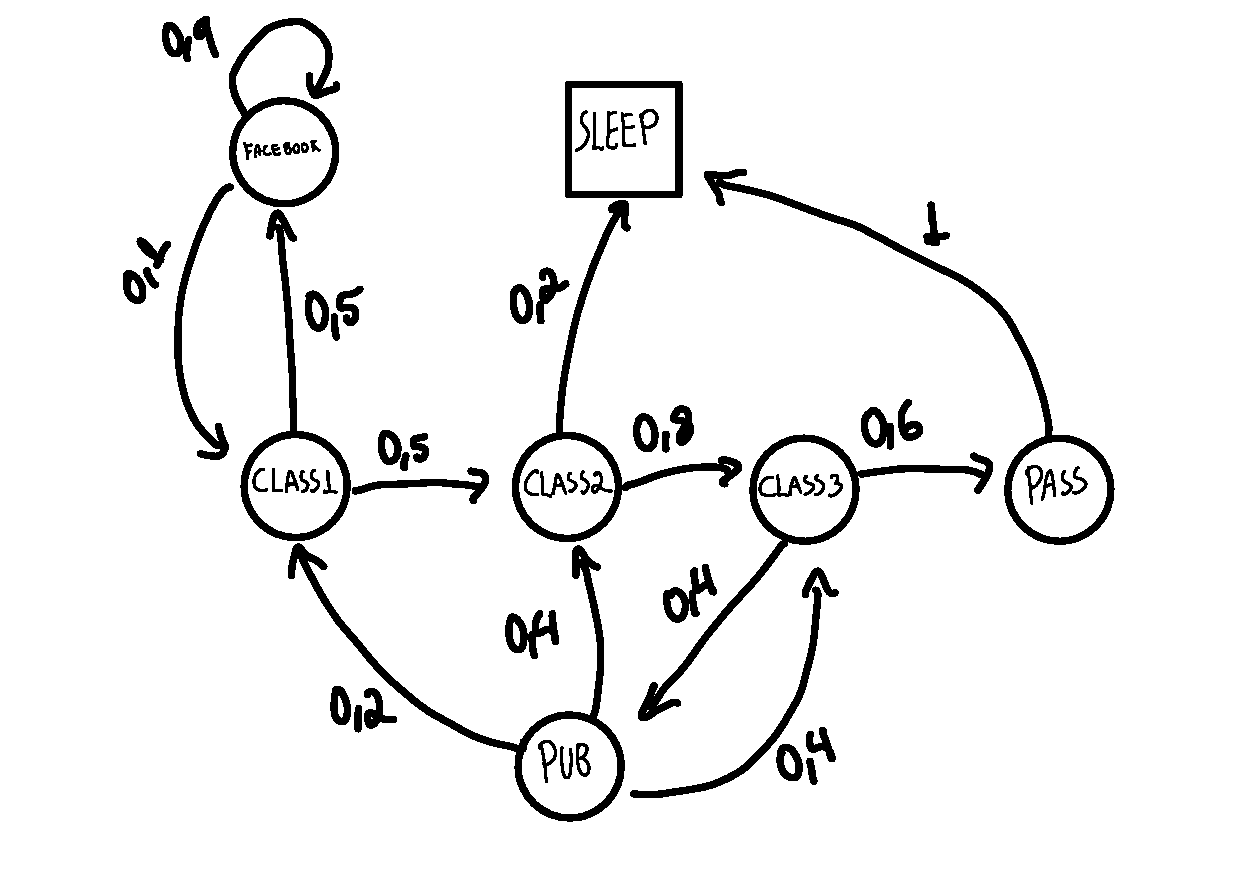
\includegraphics[width=0.9\textwidth]{sections/markov/figures/student_example.pdf}
    \end{figure}
\end{frame}

\begin{frame}
    \frametitle{Value Function (Example)}
    \begin{figure}
        \centering
        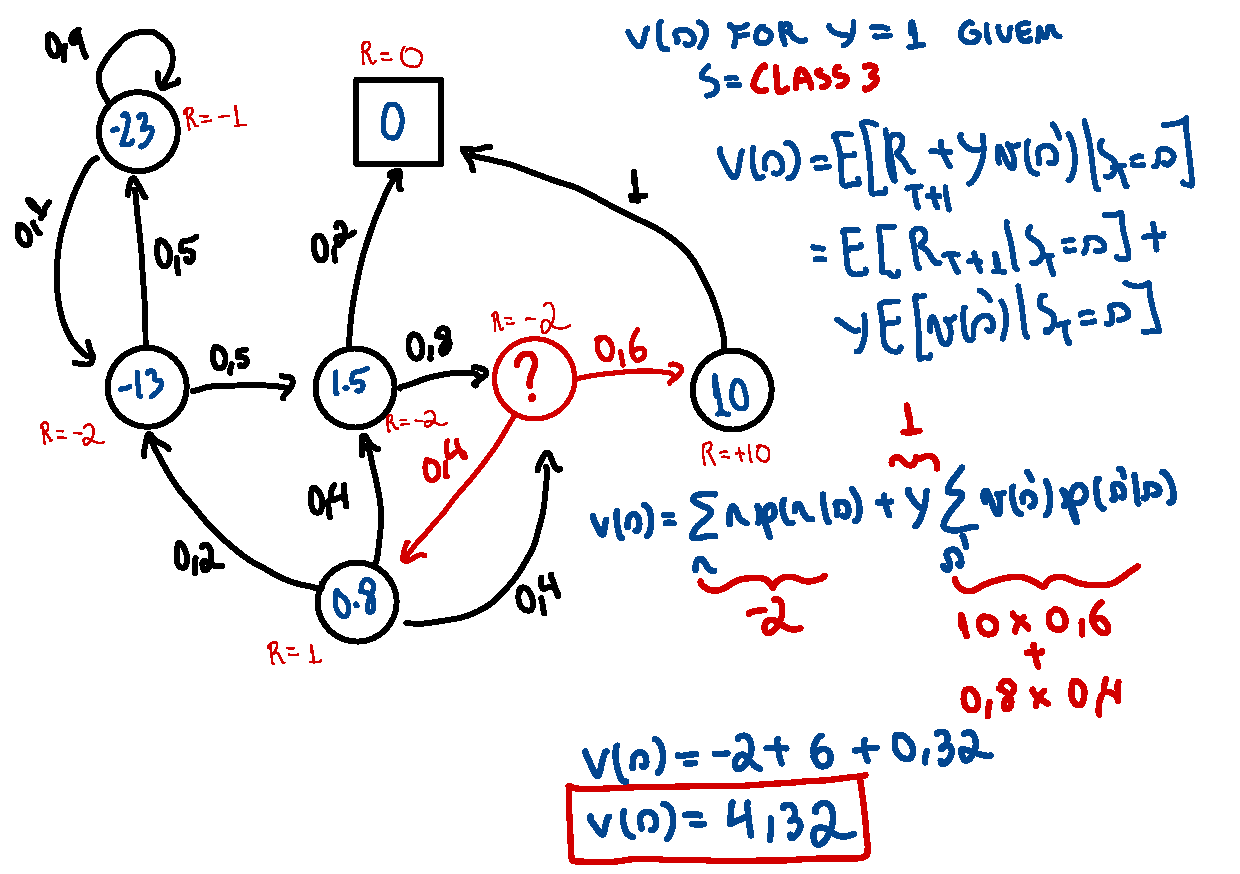
\includegraphics[width=0.9\textwidth]{sections/markov/figures/student_example_calc_v_s.pdf}
    \end{figure}
\end{frame}

\subsection{Markov Decision Process}

\begin{frame}
    \frametitle{Markov Decision Process}

    A Markov decision process (MDP) is a Markov reward process with decision (actions).
    It is an environment in which all states are Markov.

    \begin{definition}
        A Markov Decision Process is a tuple $\langle\mathcal{S},\mathcal{A},\mathcal{P},\mathcal{R},\gamma\rangle$
        \begin{itemize}
            \item $\mathcal{S}$ is a finite set of states;
            \item $\mathcal{A}$ is a finite {\color{red}set of actions};
            \item $\mathcal{P}$ is a state transition probability matrix;
            \item $\mathcal{R}$ is a reward function ($\mathcal{R}^{a}_{s}=\E[R_{t+1}|S_t=s,A_t=a]$);
            \item $\gamma$ is a discount factor where $\gamma\in[0,1]$.
        \end{itemize}
    \end{definition}
\end{frame}



\subsubsection{Policies}
\begin{frame}
    \frametitle{Policies (1)}

    \centering
    {\color{red}A policy defines the behaviour of an agent.}

    \begin{definition}
        A policy $\pi$ is a distribution over actions given states,
        $$\pi(a|s)=P[A_t=a|S_t=s]$$
    \end{definition}

\end{frame}

\begin{frame}
    \frametitle{Policies (2)}


    \begin{itemize}
        \item State transition probability matrix: 
        $$\mathcal{P}_{ss'} = P(s'|s) \rightarrow 
        {\color{red}\mathcal{P}_{ss'}^{\pi} = \sum_{a\in\mathcal{A}}\pi(a|s)P(s'|s,a)}$$
        \item Reward function: 
        $$\mathcal{R}_s = \E[R_{t+1}|S_t=s] \rightarrow 
        {\color{red}\mathcal{R}_{s}^{\pi} = \sum_{a\in\mathcal{A}}\pi(a|s)\E[R_{t+1}|S_t=s, A_t=a]}$$

        \item $\mathcal{R}_{s}^{\pi}$ can be write as:

        $$\sum_{a\in\mathcal{A}}\pi(a|s){\color{red}\E[R_{t+1}|S_t=s, A_t=a]} = 
        \sum_{a\in\mathcal{A}}\sum_{r\in\mathcal{R}}r\pi(a|s)P(r|s,a)$$
    \end{itemize}  

\end{frame}



\subsubsection{Value Functions}

\begin{frame}
    \frametitle{Value Function (Following some Policy)}
    \begin{definition}
        The state-value function $v_{\pi}(s)$ of an MDP is 
        the {\color{red} the expected return starting from $s$, and
        following some policy $\pi$}.
        $$v_{\pi}(s) = \E[G_t|S_t=s]$$
    \end{definition}


    \begin{definition}
        The action-value function $q_{\pi}(s)$ is the {\color{red} expected 
        return starting from $s$, taking action $a$ and then Following
        policy $\pi$}.
        $$q_{\pi}(s) = \E[G_t|S_t=s,A_t=a]$$
    \end{definition}

\end{frame}


\begin{frame}
    \frametitle{Backup Diagrams}
    \centering
    Backup diagram gives a visual representation of different algorithm and models in Reinforcement Learning.
    \begin{figure}
        \centering
        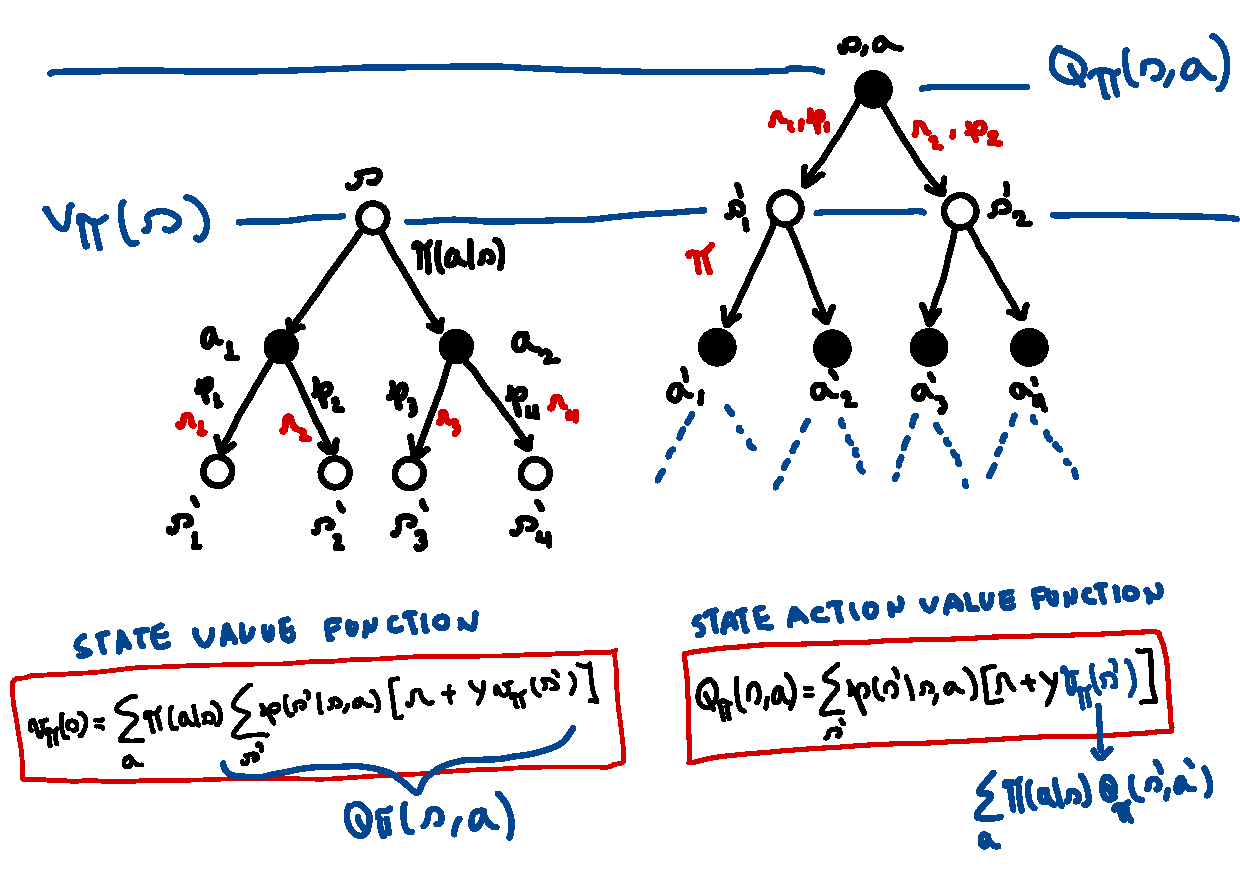
\includegraphics[width=0.8\textwidth]{sections/markov/figures/backup_diagram.pdf}
    \end{figure}
\end{frame}


\begin{frame}
    \frametitle{Value Function (Following some Policy)}
    \begin{itemize}
        \item $q$ from $v$:
        $$q_{\pi}(s,a) = \sum_{s'\in\mathcal{S}}[\mathcal{R}_{s}^{a}+\gamma~v_{\pi}(s')]$$
        \item $s$ from $q$:
        $$v_{\pi}(s) = \sum_{a\in\mathcal{A}}\pi(a|s)q_{\pi}(s,a)$$
    \end{itemize}
\end{frame}

%\begin{frame}
%    \frametitle{Bellman Expectation Equation (Matrix Form)}
%    The Bellman expectation equation can be expressed as matrix form:
%    $$v_{\pi} = \mathcal{R}_{\pi} + \gamma\mathcal{P}_{\pi}v_{\pi}$$
%    with diect solution:
%    $$v_{\pi} = (I-\gamma\mathcal{P}_{\pi})^{-1}\mathcal{R}_{\pi}$$
%\end{frame}

\subsection{Optimal Value Function}


\begin{frame}
    \frametitle{Optimal Value Function}
    \centering
    An MDP is solved when we know the optimal value function.
    \begin{definition}
        The optimal state-value function $v_{*}(s)$ is the maximum value
        function over all policies
        $$v_{*}(s) = max_{\pi}v_{\pi}(s)$$

        The optimal action-value function $q_{*}(s,a)$ is the maximum
        action-value function over all policies
        $$q_{*}(s,a) = max_{\pi}q_{\pi}(s,a)$$
    \end{definition}
\end{frame}

\begin{frame}
    \frametitle{Optimal Policy}
    \centering
    An MDP is solved when we know the optimal value function.
    \begin{definition}
        For any Markov Decision Process
        \begin{itemize}
            \item The exists an optimal policy $\pi_{*}$ that is better than
            or equal to all other policies, $\pi_{*} \geqslant \pi \forall\pi$;
            \item all optimal policies achieve the optimal value function:
            $$v_{\pi_{*}}(s) = v_{*}(s)$$
            \item all optimal policies achieve the option action-value function (Q-value):
            $$q_{\pi_{*}}(s,a) = q_{*}(s,a)$$
        \end{itemize}
    \end{definition}
\end{frame}



\begin{frame}
    \frametitle{Finding the Optimal Policy}
    An optimal policy can be found by maximising over $q_{*}(s,a)$,
    $$\pi_{*} =  \begin{cases}
        1, & \text{if}\ a=argmax(q_{*}(s,a)), \forall~a\in\mathcal{A}\\
        0, & \text{otherwise}
      \end{cases}$$

    \begin{itemize}
        \item There is always a {\color{red}deterministic} optimal policy for any MDP;
        \item If we know $q_{a}(s,a)$, we immediately have the optimal policy. 
    \end{itemize}
\end{frame}


\begin{frame}
    \frametitle{Optimal Bellman Equation for $V_{*}$}
    \begin{figure}
        \centering
        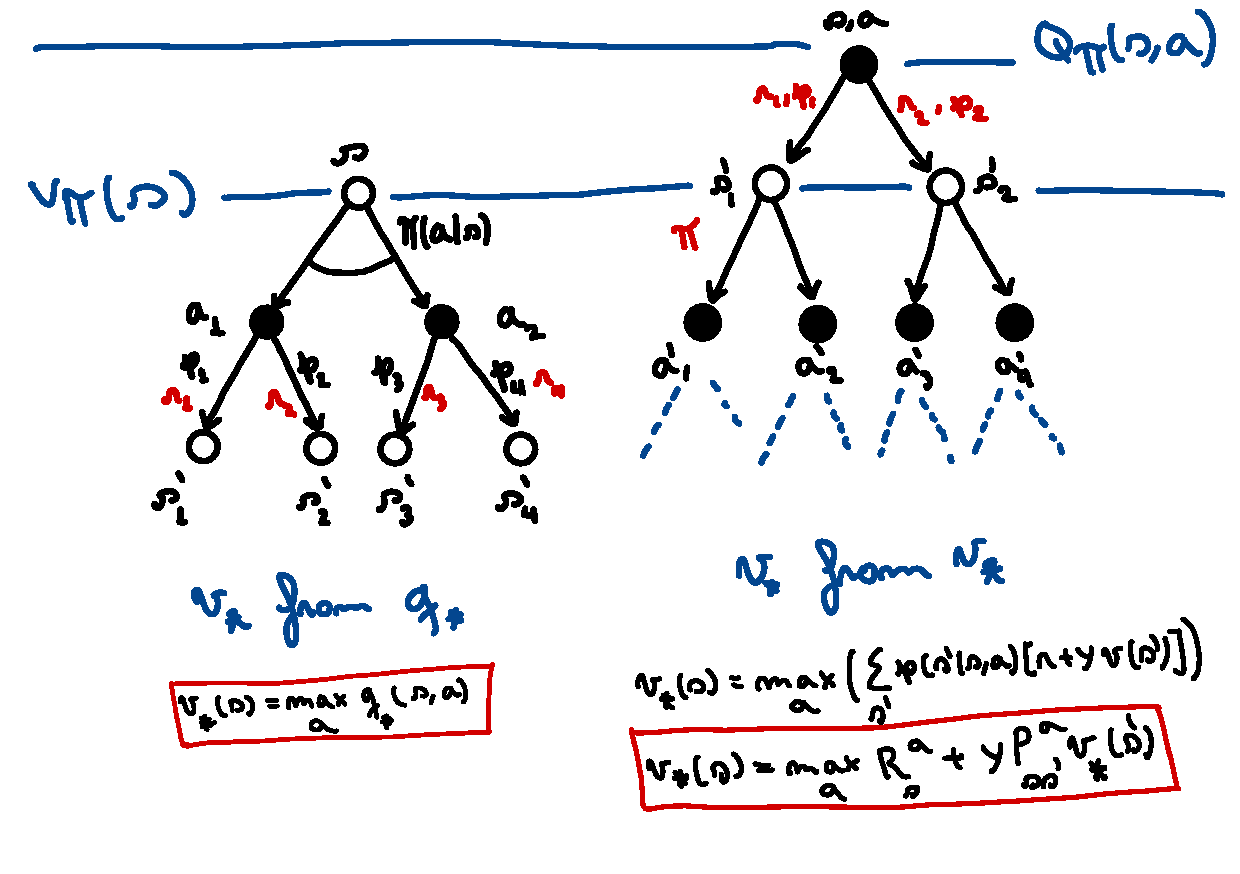
\includegraphics[width=1\textwidth]{sections/markov/figures/v_star.pdf}
    \end{figure}
\end{frame}



\begin{frame}
    \frametitle{Optimal Bellman Equation for $Q_{*}$}
    \begin{figure}
        \centering
        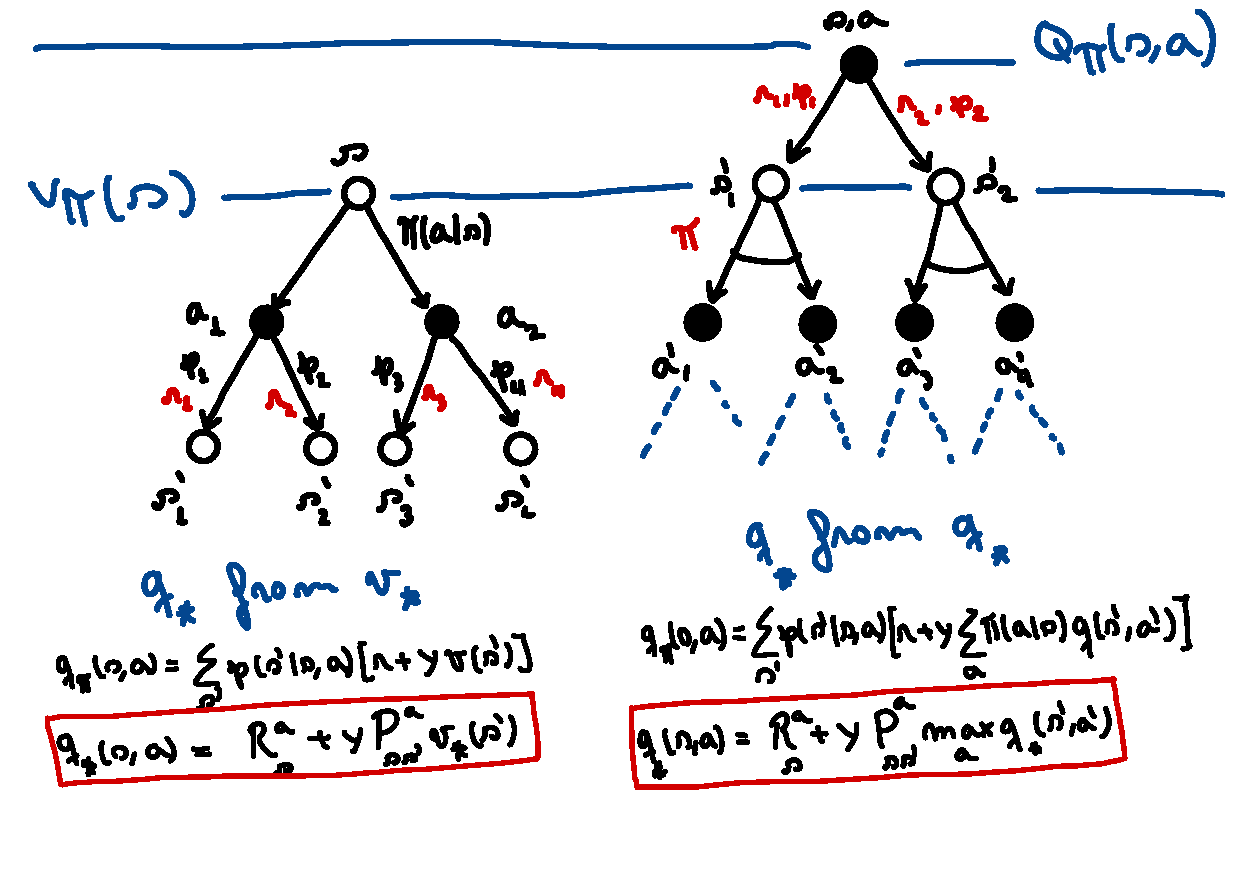
\includegraphics[width=1\textwidth]{sections/markov/figures/q_star.pdf}
    \end{figure}
\end{frame}